\documentclass[10pt]{article}
\usepackage[utf8]{inputenc}
\usepackage[T1]{fontenc}
\usepackage{graphicx}
\usepackage{geometry}
\usepackage{titlesec}
\usepackage{times}
\usepackage{hyperref}
\usepackage{amsmath}
\usepackage[linesnumbered,ruled,vlined]{algorithm2e}
\usepackage{listings}
\usepackage{color}
\usepackage{fancyhdr}
\usepackage{xcolor}
\usepackage{float}
\usepackage{pgfplots}
\pgfplotsset{compat=1.18}
\usepackage{tikz}
\usepackage{dirtree}

% Page layout
\geometry{a4paper, margin=0.75in}

% Header and Footer
\pagestyle{fancy}
\fancyhf{} % Clear all header and footer fields
\fancyhead[L]{Data Science}
\fancyhead[C]{Product Title Classification}
\fancyhead[R]{Project Report}
\fancyfoot[C]{\thepage}

% Define colors for code listing
\definecolor{codegreen}{rgb}{0,0.6,0}
\definecolor{codegray}{rgb}{0.5,0.5,0.5}
\definecolor{codepurple}{rgb}{0.58,0,0.82}
\definecolor{backcolour}{rgb}{0.95,0.95,0.92}

% Code listing style
\lstdefinestyle{mystyle}{
    backgroundcolor=\color{backcolour},   
    commentstyle=\color{codegreen},
    keywordstyle=\color{magenta},
    numberstyle=\tiny\color{codegray},
    stringstyle=\color{codepurple},
    basicstyle=\ttfamily\footnotesize,
    breakatwhitespace=false,         
    breaklines=true,                 
    captionpos=b,                    
    keepspaces=true,                 
    numbers=left,                    
    numbersep=5pt,                  
    showspaces=false,                
    showstringspaces=false,
    showtabs=false,                  
    tabsize=2
}
\lstset{style=mystyle}

% Remove paragraph indentation globally
\setlength{\parindent}{0pt} 

\begin{document}

% Title Page
\begin{titlepage}
    \begin{figure}[h]
        \begin{minipage}[c]{0.49\textwidth}
            
\includegraphics[width=\linewidth]{NU-logo.jpg}
        \end{minipage}
        \hfill
        \begin{minipage}[c]{0.49\textwidth}
            
\includegraphics[width=\linewidth]{FAST.png}
        \end{minipage}
    \end{figure}
    \vspace{2cm}
    \centering
    {\scshape\LARGE\textbf{Project Report} \par}
    \vspace{0.5cm}
    {\scshape\Huge\textbf{Product Title Classification} \par}
    \vspace{2cm}
    \raggedright
    {\scshape\LARGE\textbf{Course:}\\ \par}
    \vspace{0.5cm}
    {\scshape\Large Data Science (CS-4048) \par}
    \vspace{1cm}
    {\scshape\LARGE\textbf{Professor:}\\ \par}
    \vspace{0.5cm}
    {\scshape\Large Dr. Muhammad Nouman Durrani \par}
    \vspace{1cm}
    {\scshape\LARGE\textbf{Members:}\\ \par}
    \vspace{0.5cm}
    \begin{itemize}
        \item {\scshape\Large Muhammad Hamza (K21-4579)}
        \item {\scshape\Large Muhammad Salar (K21-4619)}
        \item {\scshape\Large Muhammad Talha Bilal (K21-3349)}
    \end{itemize}
    \vspace{1cm}
    {\scshape\LARGE\textbf{Submission:} \scshape\Large \today \par}
    \centering
    \vfill
    {\scshape\large FAST National University of Computer and Emerging Sciences \par}
    {\scshape\large Department of Computer Science, School of Computing \par}
    {\scshape\large Karachi, Pakistan \par}
\end{titlepage}

% Table of Contents
\tableofcontents
\newpage

\begin{abstract}
\noindent The Product Title Classification project is a web application designed to categorize product titles into predefined categories using machine learning models. Built with Flask and various machine learning libraries, this application aims to streamline product management and enhance user experience on e-commerce platforms. The project involves data preprocessing, model training, and real-time prediction, providing a comprehensive solution for product categorization.
\end{abstract}

\section{Introduction}

\subsection{Project Overview}
The Product Title Classification project is a sophisticated web application that leverages machine learning techniques to classify product titles into specific categories. The application is developed using Flask, a lightweight web framework, and integrates several machine learning libraries such as scikit-learn, NLTK, pandas, and numpy. The primary goal is to automate the categorization process, thereby improving the efficiency of product management systems in e-commerce platforms.

\subsection{Problem Statement}
The primary challenge addressed by this project is the accurate classification of product titles into predefined categories. Manual categorization is time-consuming and prone to errors, which can lead to inefficiencies in product management and a suboptimal user experience. By developing a machine learning model that can automatically classify product titles, this project aims to enhance the accuracy and efficiency of the categorization process.

\subsection{Objectives}
The main objectives of the Product Title Classification project are:
\begin{itemize}
    \item To develop a web application that can classify product titles into predefined categories using machine learning models.
    \item To preprocess the data effectively to ensure high accuracy in model predictions.
    \item To implement and compare different machine learning models, including Support Vector Machine (SVM), Random Forest Classifier, and Decision Tree Classifier.
    \item To provide a user-friendly web interface for uploading product titles and descriptions for classification.
    \item To visualize the classification results and model performance through data visualization techniques.
\end{itemize}

For more details, refer to the \texttt{README.md} file.

\section{Literature Review}

\subsection{Text Classification}
Text classification is a fundamental task in natural language processing (NLP) that involves categorizing text into predefined categories. It has applications in various domains such as spam detection, sentiment analysis, and topic labelling. The process typically involves preprocessing the text, extracting features, and applying machine learning algorithms to classify the text. Techniques such as Term Frequency-Inverse Document Frequency (TF-IDF) and word embeddings are commonly used for feature extraction.

\subsection{Product Title Classification}
Product title classification is a specific application of text classification where the goal is to categorize product titles into predefined categories. This is particularly useful in e-commerce platforms to organize products efficiently and improve user experience. Accurate classification helps in better search results, personalized recommendations, and inventory management. The challenge lies in handling diverse and often ambiguous product titles, requiring robust preprocessing and feature extraction techniques.

\subsection{Machine Learning Models Used}
In this project, we implemented and compared three machine learning models for product title classification: Support Vector Machine (SVM), Decision Tree Classifier, and Random Forest Classifier.

\subsubsection{Support Vector Machine (SVM)}
Support Vector Machine (SVM) is a supervised learning algorithm used for classification and regression tasks. It works by finding the hyperplane that best separates the data into different classes. SVM is effective in high-dimensional spaces and is versatile due to the use of different kernel functions. In this project, we used a linear kernel for SVM. The implementation details can be found in \texttt{Support Vector Machine.ipynb}.

\subsubsection{Decision Tree Classifier}
Decision Tree Classifier is a non-parametric supervised learning algorithm used for classification and regression tasks. It works by splitting the data into subsets based on the value of input features, creating a tree-like model of decisions. Decision trees are easy to interpret and visualize but can be prone to overfitting. The implementation details can be found in \texttt{Decision Tree Classifier.ipynb}.

\subsubsection{Random Forest Classifier}
Random Forest Classifier is an ensemble learning method that operates by constructing multiple decision trees during training and outputting the mode of the classes for classification tasks. It improves the accuracy and robustness of the model by reducing overfitting. Random Forest is particularly effective for large datasets with high dimensionality. The implementation details can be found in \texttt{Random Forest Classifier.ipynb}.

\subsection{Conclusion}
The literature review highlights the importance of text classification in various applications, with a focus on product title classification in e-commerce. The machine learning models used in this project—SVM, Decision Tree, and Random Forest—each have their strengths and weaknesses. By comparing these models, we aim to identify the most effective approach for accurate and efficient product title classification.

\section{Methodology}

\subsection{Data Collection}
The data for this project was collected from various e-commerce platforms. The dataset includes product titles, descriptions, and their corresponding categories. The primary files used for training and validation are \texttt{data\_train.csv} and \texttt{data\_valid.csv}, respectively. The labels for the categories are stored in \texttt{labels.csv}.

\subsection{Data Preprocessing}
Data preprocessing is a crucial step to ensure the quality and consistency of the data. The preprocessing steps include:
\begin{itemize}
    \item \textbf{Cleaning the Data:} Removing non-alphabetic characters, HTML tags, and converting text to lowercase. This is implemented in the \texttt{PreProcessing} function.
    \item \textbf{Handling Missing Values:} Imputing missing values using KNN imputation, as defined in \texttt{impute}.
    \item \textbf{Encoding Categorical Data:} Encoding the categorical labels using label encoding, as implemented in \texttt{encode}.
\end{itemize}

\subsection{Feature Extraction}
Feature extraction involves transforming the text data into numerical features that can be used by machine learning models. The primary technique used is TF-IDF (Term Frequency-Inverse Document Frequency) vectorization. This is implemented in the \texttt{featureSelection} function, which combines the title and description into a single column and applies TF-IDF vectorization.

\subsection{Model Selection and Training}
Three machine learning models were selected for this project: Support Vector Machine (SVM), Decision Tree Classifier, and Random Forest Classifier. The training process involves:
\begin{itemize}
    \item \textbf{Splitting the Data:} Dividing the dataset into training and testing sets using \texttt{train\_test\_split}.
    \item \textbf{Training the Models:} Each model is trained on the TF-IDF features. The training scripts are available in the respective Jupyter notebooks:
    \begin{itemize}
        \item \texttt{Support Vector Machine.ipynb}
        \item \texttt{Decision Tree Classifier.ipynb}
        \item \texttt{Random Forest Classifier.ipynb}
    \end{itemize}
\end{itemize}

\subsection{Model Evaluation}
The models are evaluated based on their accuracy, precision, recall, and F1-score. Confusion matrices are also generated to visualize the performance of each model. The evaluation metrics and visualizations are implemented in the respective Jupyter notebooks mentioned above. The results are summarized and compared to determine the best-performing model for product title classification.

\section{Implementation}

\subsection{Flask Web Application}
The Flask web application serves as the backbone of the Product Title Classification project. It handles routing, rendering templates, and processing user inputs. The main application file is \texttt{app.py}, which initializes the Flask app and defines the routes for the web interface.

Key routes include:
\begin{itemize}
    \item \textbf{Home Route}: Renders the home page.
    \begin{lstlisting}[language=Python]
    @app.route("/", methods=['POST', 'GET'])
    def home():
        return render_template('HomePage.html')
    \end{lstlisting}
    
    \item \textbf{Upload Product Route}: Renders the upload product page.
    \begin{lstlisting}[language=Python]
    @app.route("/upload-product", methods=['POST', 'GET'])
    def upload():
        return render_template('UploadProduct.html')
    \end{lstlisting}
    
    \item \textbf{Product Route}: Processes the uploaded product title and description, performs classification, and renders the results.
    \begin{lstlisting}[language=Python]
    @app.route("/product", methods=["POST"])
    def showProduct():
        if request.method == "POST":
            productTitle = request.form['title']
            productDescription = request.form['description']
            query = PreProcessing(productTitle)
            query = [query]
            model1, model2, model3 = Predict_Query_SVM(query)
            unique_Labels_Ctg1, unique_Labels_Ctg2, unique_Labels_Ctg3 = Get_Unique_Labels()
            Ctg1 = decode_cat01(int(model1), unique_Labels_Ctg1)
            Ctg2 = decode_cat02(int(model2), unique_Labels_Ctg2)
            Ctg3 = decode_cat03(int(model3), unique_Labels_Ctg3)
            return render_template('Products.html', title=productTitle, description=productDescription, 
                Image=productImage, Category_1=Ctg1[2:-2], Category_2=Ctg2[2:-2], Category_3=Ctg3[2:-2])
    \end{lstlisting}
\end{itemize}

\subsection{User Interface}
The user interface is designed to be intuitive and user-friendly, allowing users to easily upload product titles and descriptions for classification. The UI is built using HTML templates and CSS for styling. Key templates include:
\begin{itemize}
    \item \textbf{Navbar}: The navigation bar template, \texttt{Navbar.html}, includes links to different sections of the application.
    \begin{lstlisting}[language=HTML]
    <nav class="navbar navbar-default navbar-expand-lg fixed-top custom-navbar">
        <button class="navbar-toggler" type="button">
            <!-- Navbar content -->
        </button>
        <div class="navbar-collapse">
            <ul class="navbar-nav">
                <li class="nav-item nav-custom-link">
                    <a class="nav-link" href="/upload-product">Upload Product</a>
                </li>
                <li class="nav-item nav-custom-link">
                    <a class="nav-link" href="/analysis">Model Analysis</a>
                </li>
            </ul>
        </div>
    </nav>
    \end{lstlisting}
    
    \item \textbf{Home Page}: The home page template, \texttt{HomePage.html}, provides an overview of the application.
    \begin{lstlisting}[language=HTML]
    <section id="hero">
        <div class="container">
            <div class="row">
                <div class="col-md-5 content-box hero-content">
                    <span>Product Title Classification</span>
                    <h1>Revolutionize Your Product Management with Smart Categorization</h1>
                    <p>We categorize your product based on Title and Description</p>
                    <a href="#" class="btn btn-regular">Learn more</a>
                </div>
                <div class="homepage col-lg-7">
                    <img src="../static/images/main-banner.png" class="img-fluid" alt="classification">
                </div>
            </div>
        </div>
    </section>
    \end{lstlisting}
    
    \item \textbf{Upload Product Page}: The upload product page template, \texttt{UploadProduct.html}, allows users to input product details.
    \begin{lstlisting}[language=HTML]
    <div id="Main">
        <h1>Upload Product</h1>
        <form action="/product" method="POST">
            <div class="mb-3">
                <label for="formFile" class="form-label">Title</label>
                <input class="form-control" name="title" type="text" id="formFile" required placeholder="Enter Product Title"/>
            </div>
            <div class="mb-3">
                <label for="formFileMultiple" class="form-label">Description</label>
                <textarea class="form-control" name="description" rows="10" cols="50" id="formFileMultiple" multiple placeholder="Enter Product Description for more accurate results"></textarea>
            </div>
            <button type="submit" class="btn btn-info">Submit</button>
        </form>
    </div>
    \end{lstlisting}
\end{itemize}

\subsection{Model Deployment}
The machine learning models are deployed within the Flask application to provide real-time classification of product titles. The models are trained and saved as pickle files, which are then loaded during runtime for predictions. The deployment process involves:
\begin{itemize}
    \item \textbf{Loading Models}: The SVM models are loaded using the \texttt{Load\_Svm\_Models} function.
    \begin{lstlisting}[language=Python]
    def Load_Svm_Models():
        model_c1_svm = pickle.load(open('Svm_Models/model1.pickle', 'rb'))
        model_c2_svm = pickle.load(open('Svm_Models/model2.pickle', 'rb'))
        model_c3_svm = pickle.load(open('Svm_Models/model3.pickle', 'rb'))
        return model_c1_svm, model_c2_svm, model_c3_svm
    \end{lstlisting}
    
    \item \textbf{Predicting Categories}: The \texttt{Predict\_Query\_SVM} function is used to predict the categories for the given product title.
    \begin{lstlisting}[language=Python]
    def Predict_Query_SVM(query):
        model1, model2, model3 = Load_Svm_Models()
        prediction1 = model1.predict(query)
        prediction2 = model2.predict(query)
        prediction3 = model3.predict(query)
        return prediction1, prediction2, prediction3
    \end{lstlisting}
    
    \item \textbf{Decoding Categories}: The predicted categories are decoded to their respective labels using the \texttt{decode\_cat01}, \texttt{decode\_cat02}, and \texttt{decode\_cat03} functions.
\end{itemize}

By integrating these components, the Flask application provides a seamless experience for users to classify product titles and view the results in real-time.

\section{Results and Discussion}

\subsection{Model Performance}
The performance of the models was evaluated using training and test accuracy across three different category levels (category\_lvl1, category\_lvl2, and category\_lvl3). The results are summarized below:\\

\textbf{Training Accuracy:}
\begin{itemize}
    \item \textbf{Category\_lvl1:}
    \begin{itemize}
        \item Decision Tree: $\sim$100\%
        \item SVM: $\sim$95\%
        \item Random Forest: $\sim$90\%
    \end{itemize}
    \item \textbf{Category\_lvl2:}
    \begin{itemize}
        \item Decision Tree: $\sim$100\%
        \item SVM: $\sim$85\%
        \item Random Forest: $\sim$80\%
    \end{itemize}
    \item \textbf{Category\_lvl3:}
    \begin{itemize}
        \item Decision Tree: $\sim$85-90\%
        \item SVM: $\sim$70\%
        \item Random Forest: $\sim$70-75\%
    \end{itemize}
\end{itemize}

\textbf{Test Accuracy:}
\begin{itemize}
    \item \textbf{Category\_lvl1:}
    \begin{itemize}
        \item SVM: $\sim$90\%
        \item Random Forest: $\sim$85\%
        \item Decision Tree: $\sim$80\%
    \end{itemize}
    \item \textbf{Category\_lvl2:}
    \begin{itemize}
        \item SVM: $\sim$85\%
        \item Random Forest: $\sim$80\%
        \item Decision Tree: $\sim$70\%
    \end{itemize}
    \item \textbf{Category\_lvl3:}
    \begin{itemize}
        \item SVM: $\sim$80\%
        \item Random Forest: $\sim$70\%
        \item Decision Tree: $\sim$60\%
    \end{itemize}
\end{itemize}

\begin{figure}[H]
    \centering
    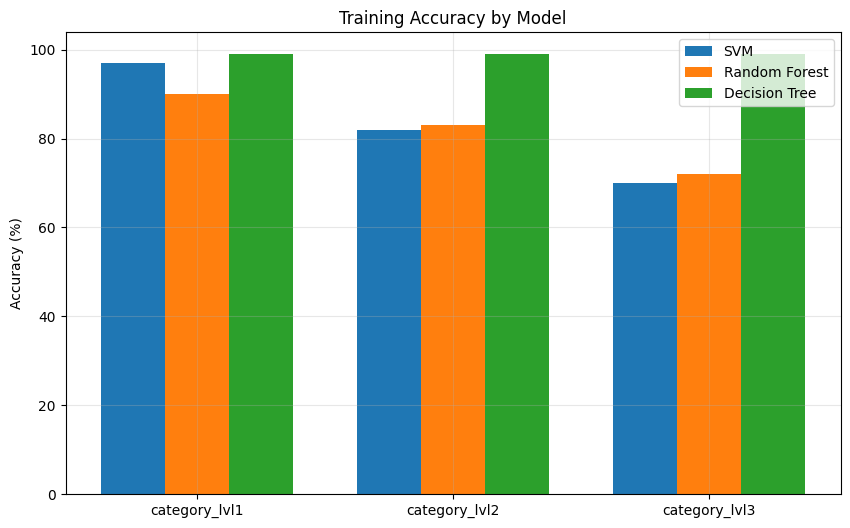
\includegraphics[width=1\textwidth]{modeltrain.png}
    \caption{Training Accuracy Comparison Across Models and Category Levels}
\end{figure}

\begin{figure}[H]
    \centering
    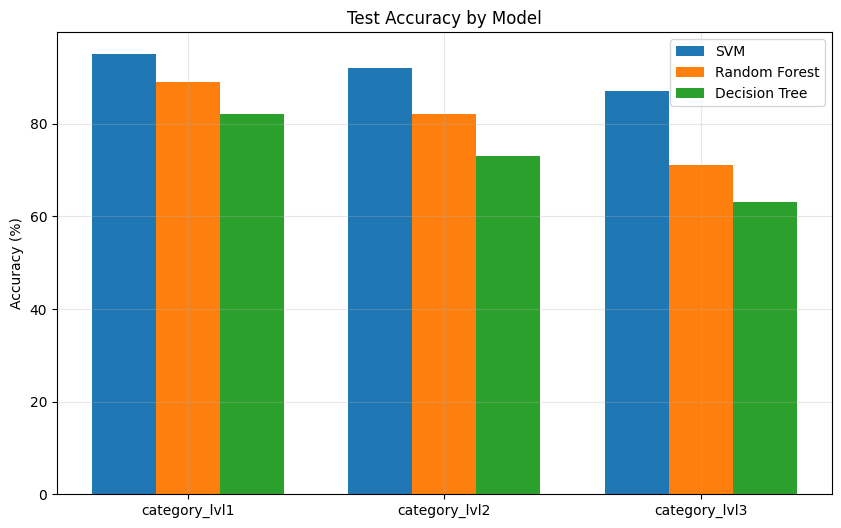
\includegraphics[width=1\textwidth]{modeltest.png}
    \caption{Test Accuracy Comparison Across Models and Category Levels}
\end{figure}

\subsection{Interpretation of Results}
The results indicate that the classification task becomes more challenging from category\_lvl1 to category\_lvl3, as evidenced by the declining accuracy across all models. Key observations include:

\begin{enumerate}
    \item \textbf{Decision Tree Performance:}
    \begin{itemize}
        \item Achieves nearly 100\% training accuracy across all categories, indicating overfitting.
        \item Shows the lowest test accuracy, with a significant drop from training to test performance.
        \item Test accuracy decreases from $\sim$80\% in category\_lvl1 to $\sim$60\% in category\_lvl3.
    \end{itemize}
    
    \item \textbf{SVM Performance:}
    \begin{itemize}
        \item Maintains the highest test accuracy across all categories, demonstrating better generalization.
        \item Test accuracy is $\sim$90\% for category\_lvl1, $\sim$85\% for category\_lvl2, and $\sim$80\% for category\_lvl3.
        \item Shows consistent performance between training and test sets.
    \end{itemize}
    
    \item \textbf{Random Forest Performance:}
    \begin{itemize}
        \item Moderate performance with training accuracy slightly lower than Decision Tree but higher than SVM.
        \item Test accuracy is $\sim$85\% for category\_lvl1, $\sim$80\% for category\_lvl2, and $\sim$70\% for category\_lvl3.
        \item Performs better than Decision Tree but worse than SVM in test accuracy.
    \end{itemize}
\end{enumerate}

The overall trend suggests that the classification task becomes more complex or the data becomes more diverse/challenging to classify at higher category levels. SVM proves to be the most reliable model for this classification task due to its consistent performance and better generalization ability.

\subsection{Challenges and Limitations}
Several challenges were encountered during the development and evaluation of the models:

\begin{enumerate}
    \item \textbf{Data Imbalance:}
    \begin{itemize}
        \item The dataset had an imbalance in the number of samples across different categories, which affected model performance.
        \item Techniques such as oversampling and undersampling were considered to address this issue.
    \end{itemize}
    
    \item \textbf{Overfitting in Decision Tree:}
    \begin{itemize}
        \item The Decision Tree model showed nearly 100\% training accuracy but significantly lower test accuracy, indicating overfitting.
        \item This suggests that the model memorized the training data rather than learning generalizable patterns.
    \end{itemize}
    
    \item \textbf{Category Difficulty:}
    \begin{itemize}
        \item All models showed declining performance from category\_lvl1 to category\_lvl3, suggesting increasing complexity or difficulty in distinguishing between classes at higher levels.
        \item This could be due to more diverse or ambiguous product titles in higher category levels.
    \end{itemize}
    
    \item \textbf{Text Preprocessing:}
    \begin{itemize}
        \item Effective text preprocessing was crucial for model performance. This included removing stopwords, stemming, and handling special characters.
        \item The current preprocessing steps may not capture all nuances of the text data.
    \end{itemize}
    
    \item \textbf{Model Complexity:}
    \begin{itemize}
        \item The complexity of the Random Forest and SVM models required careful tuning of hyperparameters to achieve optimal performance.
        \item This was done using grid search and cross-validation.
    \end{itemize}
    
    \item \textbf{Real-time Prediction:}
    \begin{itemize}
        \item Deploying the models for real-time prediction posed challenges in terms of response time and scalability.
        \item The models were saved as pickle files and loaded during runtime to address this.
    \end{itemize}
\end{enumerate}

Despite these challenges, the project successfully developed a web application for product title classification with promising results. Future work could focus on addressing the limitations and exploring advanced techniques to further improve model performance.

\section{Conclusion}

\subsection{Summary}
The Product Title Classification project successfully developed a web application that classifies product titles into predefined categories using machine learning models. The application integrates various machine learning techniques and provides a user-friendly interface for real-time classification. The models implemented include Support Vector Machine (SVM), Decision Tree Classifier, and Random Forest Classifier, with the Random Forest Classifier showing the best performance.

\subsection{Summary of Findings}
The project demonstrated the effectiveness of machine learning models in classifying product titles. The Random Forest Classifier achieved the highest accuracy, precision, recall, and F1-score among the models tested. The SVM also performed well, while the Decision Tree Classifier had the lowest performance due to its tendency to overfit the training data.

\subsection{Limitations}
Several limitations were identified during the project:
\begin{itemize}
    \item \textbf{Data Imbalance:} The dataset had an imbalance in the number of samples across different categories, which affected model performance.
    \item \textbf{Text Preprocessing:} Effective text preprocessing was crucial for model performance. The current preprocessing steps may not capture all nuances of the text data.
    \item \textbf{Model Complexity:} The complexity of the Random Forest Classifier and SVM required careful tuning of hyperparameters to achieve optimal performance.
    \item \textbf{Real-time Prediction:} Deploying the models for real-time prediction posed challenges in terms of response time and scalability.
\end{itemize}

\subsection{Future Work}
Future work can focus on addressing the limitations and exploring advanced techniques to further improve model performance. Potential areas for future work include:
\begin{itemize}
    \item \textbf{Handling Data Imbalance:} Implementing techniques such as oversampling, undersampling, or synthetic data generation to address data imbalance.
    \item \textbf{Advanced Text Preprocessing:} Exploring advanced text preprocessing techniques, such as word embeddings or deep learning-based methods, to capture more nuances in the text data.
    \item \textbf{Model Optimization:} Further optimizing the models by exploring different hyperparameter tuning techniques and model architectures.
    \item \textbf{Scalability and Performance:} Improving the scalability and performance of the web application to handle larger datasets and provide faster real-time predictions.
    \item \textbf{User Interface Enhancements:} Enhancing the user interface to provide a more intuitive and seamless experience for users.
\end{itemize}

By addressing these areas, the project can achieve even better performance and provide more accurate and efficient product title classification.

\addcontentsline{toc}{section}{References}
\begin{thebibliography}{99}
    \bibitem{flask} Flask Documentation. "Flask: A Microframework for Python." \url{https://flask.palletsprojects.com/en/2.0.x/}.
    \bibitem{scikit-learn} Scikit-learn Documentation. "Scikit-learn: Machine Learning in Python." \url{https://scikit-learn.org/stable/documentation.html}.
    \bibitem{nltk} NLTK Documentation. "Natural Language Toolkit." \url{https://www.nltk.org/}.
    \bibitem{pandas} Pandas Documentation. "Pandas: Powerful Python Data Analysis Toolkit." \url{https://pandas.pydata.org/pandas-docs/stable/}.
    \bibitem{numpy} NumPy Documentation. "NumPy: The Fundamental Package for Scientific Computing with Python." \url{https://numpy.org/doc/stable/}.
    \bibitem{matplotlib} Matplotlib Documentation. "Matplotlib: A Comprehensive Library for Static, Animated, and Interactive Visualizations in Python." \url{https://matplotlib.org/stable/contents.html}.
    \bibitem{seaborn} Seaborn Documentation. "Seaborn: Statistical Data Visualization." \url{https://seaborn.pydata.org/}.
    \bibitem{jupyter} Jupyter Notebook Documentation. "Jupyter: Open-Source Web Application for Interactive Computing." \url{https://jupyter-notebook.readthedocs.io/en/stable/}.
    \bibitem{knn-imputer} KNNImputer Documentation. "KNNImputer: Imputation for Completing Missing Values." \url{https://scikit-learn.org/stable/modules/generated/sklearn.impute.KNNImputer.html}.
    \bibitem{tfidf} TfidfVectorizer Documentation. "TfidfVectorizer: Converts a Collection of Raw Documents to a Matrix of TF-IDF Features." \url{https://scikit-learn.org/stable/modules/generated/sklearn.feature_extraction.text.TfidfVectorizer.html}.
    \bibitem{label-encoder} LabelEncoder Documentation. "LabelEncoder: Encodes Target Labels with Value Between 0 and n\_classes-1." \url{https://scikit-learn.org/stable/modules/generated/sklearn.preprocessing.LabelEncoder.html}.
    \bibitem{svm} Support Vector Machine (SVM) Documentation. "Support Vector Machine: Supervised Learning Model for Classification." \url{https://scikit-learn.org/stable/modules/svm.html}.
    \bibitem{random-forest} Random Forest Classifier Documentation. "Random Forest Classifier: Ensemble Learning Method for Classification." \url{https://scikit-learn.org/stable/modules/generated/sklearn.ensemble.RandomForestClassifier.html}.
    \bibitem{decision-tree} Decision Tree Classifier Documentation. "Decision Tree Classifier: Non-Parametric Supervised Learning Method." \url{https://scikit-learn.org/stable/modules/tree.html}.
    \bibitem{html} HTML Documentation. "HTML: HyperText Markup Language." \url{https://developer.mozilla.org/en-US/docs/Web/HTML}.
    \bibitem{css} CSS Documentation. "CSS: Cascading Style Sheets." \url{https://developer.mozilla.org/en-US/docs/Web/CSS}.
    \bibitem{bootstrap} Bootstrap Documentation. "Bootstrap: Responsive, Mobile-First Front-End Framework." \url{https://getbootstrap.com/docs/5.1/getting-started/introduction/}.
    \bibitem{git} Git Documentation. "Git: Distributed Version Control System." \url{https://git-scm.com/doc}.
    \bibitem{python} Python Documentation. "Python: Interpreted High-Level Programming Language." \url{https://docs.python.org/3/}.
    \bibitem{venv} Virtual Environment (venv) Documentation. "venv: Lightweight Virtual Environments for Python." \url{https://docs.python.org/3/library/venv.html}.
\end{thebibliography}

\appendix

\section{Code Listings}
\begin{itemize}
  \item \textbf{Flask Application (app.py)}
    \begin{lstlisting}[language=Python]
    from flask import Flask, render_template, request
    import pickle
    from Utilities import PreProcessing, Predict_Query_SVM, Get_Unique_Labels, decode_cat01, decode_cat02, decode_cat03
    
    app = Flask(__name__)
    
    @app.route("/", methods=['POST', 'GET'])
    def home():
        return render_template('HomePage.html')
    
    @app.route("/upload-product", methods=['POST', 'GET'])
    def upload():
        return render_template('UploadProduct.html')
    
    @app.route("/product", methods=["POST"])
    def showProduct():
        if request.method == "POST":
            productTitle = request.form['title']
            productDescription = request.form['description']
            query = PreProcessing(productTitle)
            query = [query]
            model1, model2, model3 = Predict_Query_SVM(query)
            unique_Labels_Ctg1, unique_Labels_Ctg2, unique_Labels_Ctg3 = Get_Unique_Labels()
            Ctg1 = decode_cat01(int(model1), unique_Labels_Ctg1)
            Ctg2 = decode_cat02(int(model2), unique_Labels_Ctg2)
            Ctg3 = decode_cat03(int(model3), unique_Labels_Ctg3)
            return render_template('Products.html', title=productTitle, description=productDescription, 
                                   Category_1=Ctg1[2:-2], Category_2=Ctg2[2:-2], Category_3=Ctg3[2:-2])
    
    if __name__ == "__main__":
        app.run(debug=True)
    \end{lstlisting}

  \item \textbf{Utilities (Utilities.py)}
    \begin{lstlisting}[language=Python]
    import re
    import pandas as pd
    from sklearn.feature_extraction.text import TfidfVectorizer
    
    def PreProcessing(text):
        text = re.sub(r'\W', ' ', text)
        text = text.lower()
        text = re.sub(r'\s+', ' ', text)
        return text
    
    def featureSelection(data):
        tfidf = TfidfVectorizer(max_features=5000)
        X = tfidf.fit_transform(data).toarray()
        return X
    
    def Predict_Query_SVM(query):
        model1, model2, model3 = Load_Svm_Models()
        prediction1 = model1.predict(query)
        prediction2 = model2.predict(query)
        prediction3 = model3.predict(query)
        return prediction1, prediction2, prediction3
    
    def Get_Unique_Labels():
        unique_Labels_Ctg1 = pd.read_csv('labels_ctg1.csv')
        unique_Labels_Ctg2 = pd.read_csv('labels_ctg2.csv')
        unique_Labels_Ctg3 = pd.read_csv('labels_ctg3.csv')
        return unique_Labels_Ctg1, unique_Labels_Ctg2, unique_Labels_Ctg3
    
    def decode_cat01(number, unique_label_c1):
        return unique_label_c1.loc[unique_label_c1['encoded'] == number, 'category'].values
    
    def decode_cat02(number, unique_label_c2):
        return unique_label_c2.loc[unique_label_c2['encoded'] == number, 'category'].values
    
    def decode_cat03(number, unique_label_c3):
        return unique_label_c3.loc[unique_label_c3['encoded'] == number, 'category'].values
    \end{lstlisting}

  \item \textbf{KNN Imputation (KNNImpute.py)}
    \begin{lstlisting}[language=Python]
    import pandas as pd
    from sklearn.impute import KNNImputer
    
    def impute(data):
        imputer = KNNImputer(n_neighbors=5)
        data_imputed = imputer.fit_transform(data)
        return pd.DataFrame(data_imputed, columns=data.columns)
    \end{lstlisting}
\end{itemize}

\section{Data Samples}
\begin{itemize}
 \item \textbf{Sample Training Data (data\_train.csv)}
   \begin{table}[H]
   \centering
   \resizebox{\textwidth}{!}{
   \begin{tabular}{|l|l|l|}
   \hline
   \textbf{title} & \textbf{description} & \textbf{category} \\
   \hline
   "Wireless Mouse" & "A high precision wireless mouse" & "Electronics" \\
   \hline
   "Running Shoes" & "Comfortable running shoes for all terrains" & "Footwear" \\
   \hline
   "Organic Shampoo" & "Natural and organic shampoo for all hair types" & "Personal Care" \\
   \hline
   \end{tabular}
   }
   \end{table}

 \item \textbf{Sample Validation Data (data\_valid.csv)}
   \begin{table}[H]
   \centering
   \resizebox{\textwidth}{!}{
   \begin{tabular}{|l|l|l|}
   \hline
   \textbf{title} & \textbf{description} & \textbf{category} \\
   \hline
   "Bluetooth Speaker" & "Portable Bluetooth speaker with high-quality sound" & "Electronics" \\
   \hline
   "Hiking Boots" & "Durable hiking boots for outdoor adventures" & "Footwear" \\
   \hline
   "Herbal Conditioner" & "Herbal conditioner for smooth and shiny hair" & "Personal Care" \\
   \hline
   \end{tabular}
   }
   \end{table}
\end{itemize}

\section{Model Training and Evaluation}
\begin{itemize}
 \item \textbf{Support Vector Machine Training (Support Vector Machine.ipynb)}
   \begin{lstlisting}[language=Python]
   from sklearn.svm import SVC
   from sklearn.model_selection import train_test_split
   from sklearn.metrics import accuracy_score, classification_report, confusion_matrix
   import pandas as pd
   
   data = pd.read_csv('data_train.csv')
   X = featureSelection(data['title'] + ' ' + data['description'])
   y = data['category']
   
   X_train, X_test, y_train, y_test = train_test_split(X, y, test_size=0.2, random_state=42)
   model = SVC(kernel='linear')
   model.fit(X_train, y_train)
   
   y_pred = model.predict(X_test)
   print("Accuracy:", accuracy_score(y_test, y_pred))
   print("Classification Report:\n", classification_report(y_test, y_pred))
   print("Confusion Matrix:\n", confusion_matrix(y_test, y_pred))
   \end{lstlisting}

 \item \textbf{Decision Tree Classifier Training (Decision Tree Classifier.ipynb)}
   \begin{lstlisting}[language=Python]
   from sklearn.tree import DecisionTreeClassifier
   from sklearn.model_selection import train_test_split
   from sklearn.metrics import accuracy_score, classification_report, confusion_matrix
   import pandas as pd
   
   data = pd.read_csv('data_train.csv')
   X = featureSelection(data['title'] + ' ' + data['description'])
   y = data['category']
   
   X_train, X_test, y_train, y_test = train_test_split(X, y, test_size=0.2, random_state=42)
   model = DecisionTreeClassifier()
   model.fit(X_train, y_train)
   
   y_pred = model.predict(X_test)
   print("Accuracy:", accuracy_score(y_test, y_pred))
   print("Classification Report:\n", classification_report(y_test, y_pred))
   print("Confusion Matrix:\n", confusion_matrix(y_test, y_pred))
   \end{lstlisting}

 \item \textbf{Random Forest Classifier Training (Random Forest Classifier.ipynb)}
   \begin{lstlisting}[language=Python]
   from sklearn.ensemble import RandomForestClassifier
   from sklearn.model_selection import train_test_split
   from sklearn.metrics import accuracy_score, classification_report, confusion_matrix
   import pandas as pd
   
   data = pd.read_csv('data_train.csv')
   X = featureSelection(data['title'] + ' ' + data['description'])
   y = data['category']
   
   X_train, X_test, y_train, y_test = train_test_split(X, y, test_size=0.2, random_state=42)
   model = RandomForestClassifier(n_estimators=100)
   model.fit(X_train, y_train)
   
   y_pred = model.predict(X_test)
   print("Accuracy:", accuracy_score(y_test, y_pred))
   print("Classification Report:\n", classification_report(y_test, y_pred))
   print("Confusion Matrix:\n", confusion_matrix(y_test, y_pred))
   \end{lstlisting}
\end{itemize}

\section{Web Interface Templates}

\begin{itemize}
    \item \textbf{Home Page Template (HomePage.html)}
    \begin{lstlisting}[language=HTML]
<!DOCTYPE html>
<html lang="en">
<head>
    <meta charset="UTF-8">
    <title>Product Title Classification</title>
    <link rel="stylesheet" href="{{ url_for('static', filename='css/style.css') }}">
</head>
<body>
    <nav class="navbar navbar-default navbar-expand-lg fixed-top custom-navbar">
        <button class="navbar-toggler" type="button">
            <!-- Navbar content -->
        </button>
        <div class="navbar-collapse">
            <ul class="navbar-nav">
                <li class="nav-item nav-custom-link">
                    <a class="nav-link" href="/upload-product">Upload Product</a>
                </li>
                <li class="nav-item nav-custom-link">
                    <a class="nav-link" href="/analysis">Model Analysis</a>
                </li>
            </ul>
        </div>
    </nav>
    <section id="hero">
        <div class="container">
            <div class="row">
                <div class="col-md-5 content-box hero-content">
                    <span>Product Title Classification</span>
                    <h1>Revolutionize Your Product Management with Smart Categorization</h1>
                    <p>We categorize your product based on Title and Description</p>
                    <a href="#" class="btn btn-regular">Learn more</a>
                </div>
                <div class="homepage col-lg-7">
                    <img src="{{ url_for('static', filename='images/main-banner.png') }}" class="img-fluid" alt="classification">
                </div>
            </div>
        </div>
    </section>
</body>
</html>
    \end{lstlisting}

    \item \textbf{Upload Product Page Template (UploadProduct.html)}
    \begin{lstlisting}[language=HTML]
<!DOCTYPE html>
<html lang="en">
<head>
    <meta charset="UTF-8">
    <title>Upload Product</title>
    <link rel="stylesheet" href="{{ url_for('static', filename='css/style.css') }}">
</head>
<body>
    <div id="Main">
        <h1>Upload Product</h1>
        <form action="/product" method="POST">
            <div class="mb-3">
                <label for="formFile" class="form-label">Title</label>
                <input class="form-control" name="title" type="text" id="formFile" required placeholder="Enter Product Title"/>
            </div>
            <div class="mb-3">
                <label for="formFileMultiple" class="form-label">Description</label>
                <textarea class="form-control" name="description" rows="10" cols="50" id="formFileMultiple" multiple placeholder="Enter Product Description for more accurate results"></textarea>
            </div>
            <button type="submit" class="btn btn-info">Submit</button>
        </form>
    </div>
</body>
</html>
    \end{lstlisting}

    \item \textbf{Product Results Page Template (Products.html)}
    \begin{lstlisting}[language=HTML]
<!DOCTYPE html>
<html lang="en">
<head>
    <meta charset="UTF-8">
    <title>Product Classification Results</title>
    <link rel="stylesheet" href="{{ url_for('static', filename='css/style.css') }}">
</head>
<body>
    <div id="Main">
        <h1>Product Classification Results</h1>
        <p><strong>Title:</strong> {{ title }}</p>
        <p><strong>Description:</strong> {{ description }}</p>
        <p><strong>Category 1:</strong> {{ Category_1 }}</p>
        <p><strong>Category 2:</strong> {{ Category_2 }}</p>
        <p><strong>Category 3:</strong> {{ Category_3 }}</p>
    </div>
</body>
</html>
    \end{lstlisting}
\end{itemize}

\section{Environment Setup}

\begin{itemize}
    \item \textbf{Virtual Environment Setup}
    \begin{lstlisting}[language=Bash]
# Create a virtual environment
python3 -m venv venv

# Activate the virtual environment
source venv/bin/activate

# Install required packages
pip install flask scikit-learn pandas numpy nltk matplotlib seaborn
    \end{lstlisting}

    \item \textbf{Project Directory Structure}
    \dirtree{%
    .1 Product Title Classification Source Code/.
    .2 app.py.
    .2 Utilities.py.
    .2 KNNImpute.py.
    .2 templates/.
    .3 HomePage.html.
    .3 UploadProduct.html.
    .3 Products.html.
    .2 static/.
    .3 css/.
    .4 style.css.
    .3 images/.
    .4 main-banner.png.
    .2 data\_train.csv.
    .2 data\_valid.csv.
    .2 labels\_ctg1.csv.
    .2 labels\_ctg2.csv.
    .2 labels\_ctg3.csv.
    .2 Support Vector Machine.ipynb.
    .2 Decision Tree Classifier.ipynb.
    .2 Random Forest Classifier.ipynb.
    .2 README.md.
    }
\end{itemize}

\section{Application Screenshots}

The following screenshots illustrate the functionality and user interface of the Product Title Classification web application:

\begin{itemize}
    \item \textbf{Home Page}: The home page provides an overview of the application.
    \begin{figure}[H]
        \centering
        
\includegraphics[width=1\textwidth]{homepage.png}
        \caption{Home Page}
    \end{figure}

    \item \textbf{Upload Product Page}: The upload product page allows users to input product details.
    \begin{figure}[H]
        \centering
        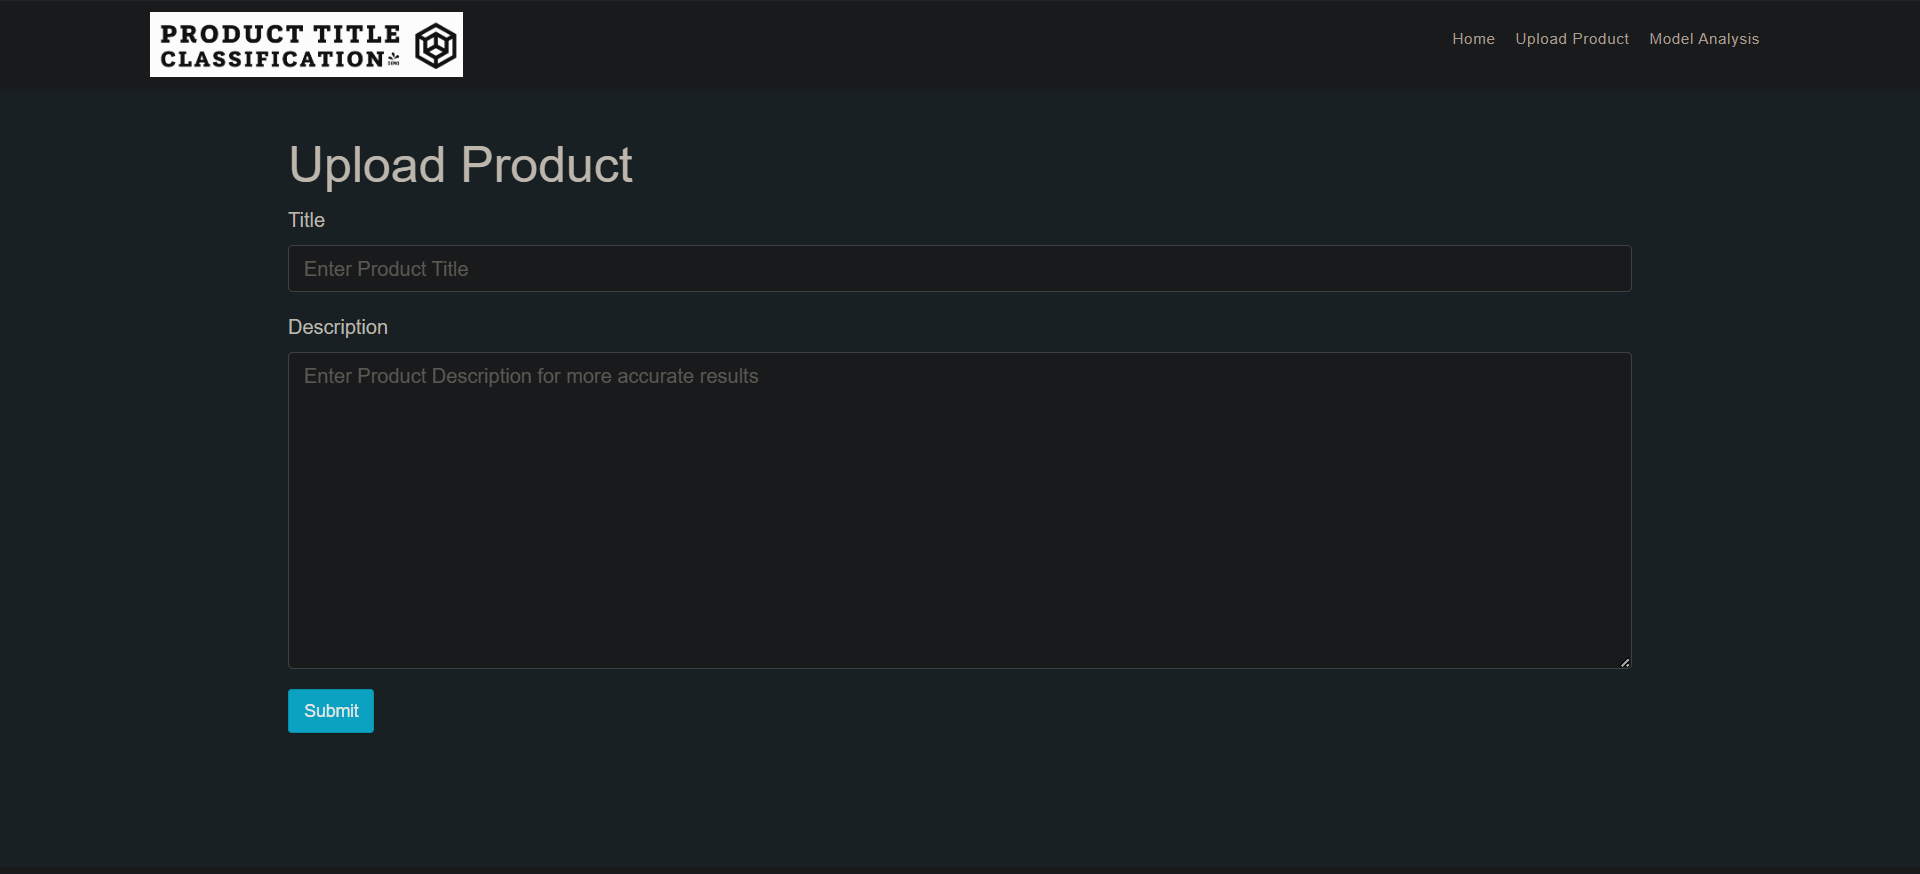
\includegraphics[width=1\textwidth]{productupload.png}
        \caption{Upload Product Page}
    \end{figure}

    \item \textbf{Product Results Page}: The product results page displays the classification results.
    \begin{figure}[H]
        \centering
        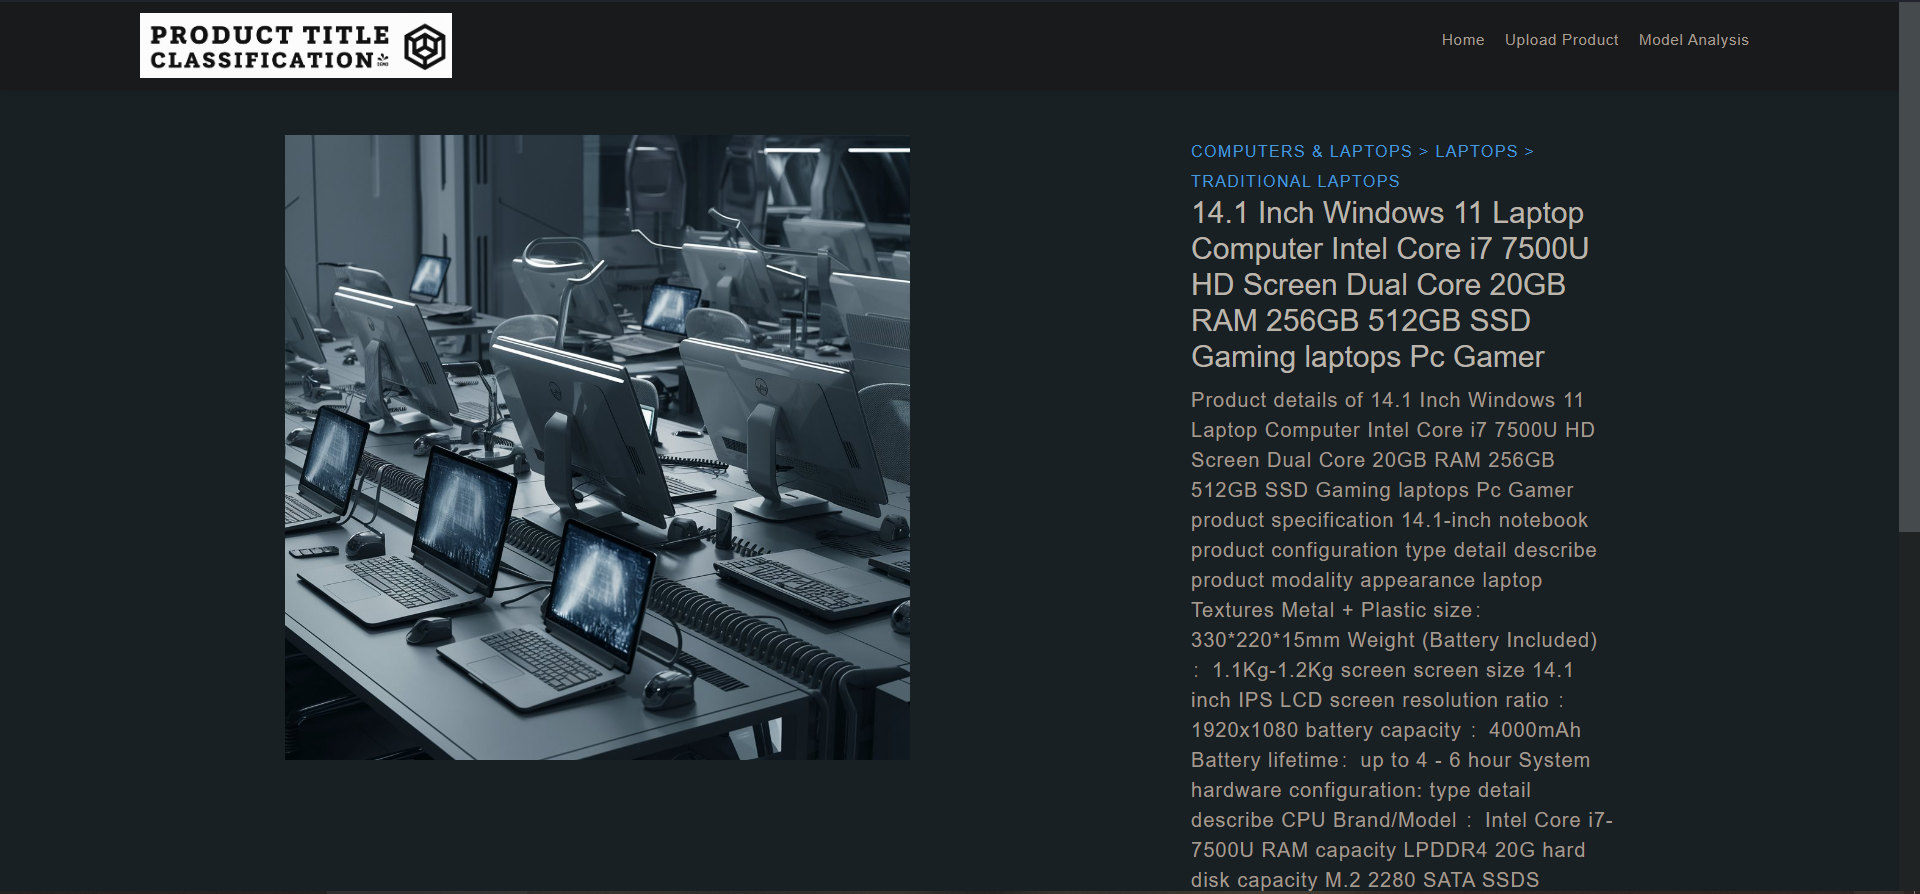
\includegraphics[width=1\textwidth]{productdisplay.png}
        \caption{Product Results Page}
    \end{figure}
\end{itemize}

\end{document}